
\documentclass[crop,tikz,border=0pt,12pt]{standalone}

\usepackage{amsthm,amsmath,latexsym,mathtools}

\definecolor{pOrange}{RGB}{211,153,80}

\begin{document}
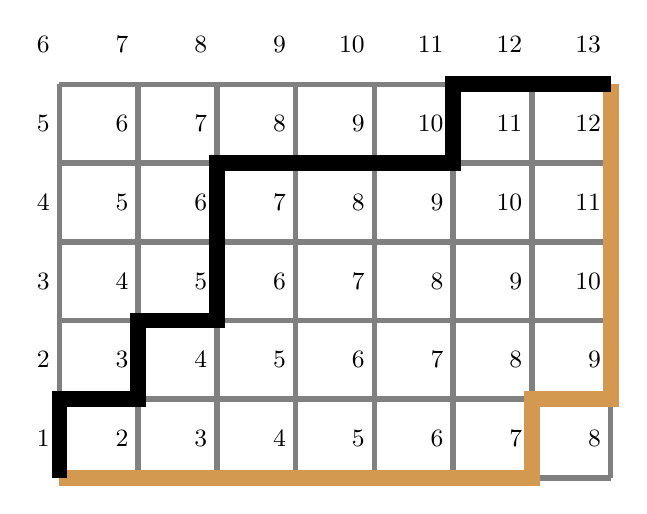
\begin{tikzpicture}
    % Draw the grid
    \foreach \x in {0,1,...,7} {
        \foreach \y in {0,1,...,5} {
            \draw[line width=0.7mm,gray] (\x,0) -- (\x,5); % Vertical lines
            \draw[line width=0.7mm,gray] (0,\y) -- (7,\y); % Horizontal lines
        }
    }
    % Label the North unit segments
    \foreach \x in {0,1,...,7} {
        \foreach \y in {0,1,...,5} {
            \node[left] at (\x,\y+0.5) {\small \the\numexpr\x+\y+1\relax};
        }
    }
     % Bottom Path
    \draw[line width=2mm, pOrange] 
        (0,0) -- (6,0) -- (6,1) -- (7,1) -- (7,5);
    
    % Top path
    \draw[line width=2mm, black] 
        (0,0) -- (0,1) -- (1,1) -- (1,2) -- (2,2) -- (2,4) -- (5,4) -- (5,5) -- (7,5);

\end{tikzpicture}
\end{document}
